

\section{Normalized Hard Sample Mining Loss}
\label{app:nhsm}
We detail the NHSM loss used in our work here.
 Formally, for the current mini-batch, the training loss is defined as
$L = LogSumExp(\lambda z(e_s, e_t)) + LogSumExp(\lambda z(e_t, e_s))$
, $e_s \in B_s$, $e_t \in B_t$, and $(e_s, e_t) \in \phi^{\prime}$
, where
$LogSumExp(X) = log(\sum_{x \in X}e^x)$
is an operator to smoothly generate hard negative samples,
$\lambda$ is the smooth factor of $LogSumExp$, and 
% This loss introduces a normalize function $l_n(e_{i}, e_{j}, e_{j}^{\prime})$, defined as follows. Formally,
% $l_{n}(e_{i}, e_{j}, e_{j}^{\prime})=\frac{l_{o}(e_{i}, e_{j}, e_{j}^{\prime})-\mu(e_{i}, e_{j})}{\sqrt{\sigma^{2}(e_{i}, e_{j})-\epsilon}}$
$z \in\mathcal{R}^{|B_t|}$ is the normalized triple loss, defined as

\vspace{-5mm}
\begin{equation}
% \begin{array}{c}
z(e_{s}, e_{t}) =\operatorname{z-score}(\{\gamma+\operatorname{sim}(e_{s}, e_{t})-\operatorname{sim}(e_{s}, e_{t}^{\prime}) | e^{\prime}_t \in B_t\}),
% \end{array}
\end{equation}
% \vspace{-2mm}
where $\operatorname{z-score}(X)=  \frac{X - \mu(X)}{\sigma(X)}$ is the standard score normalization,
and $\operatorname{sim}(e_{s}, e_{t})= \mathbf{h}_{e_s} \cdot \mathbf{h}_{e_t}$ is the similarity of two entities obtained with the GNN output feature.



\section{Adjacency Matrix Construction for \MetisGCN{}}
\label{app:adj-matrix}
Following~\cite{GCN-Align18}, to construct the adjacency matrix $A \in R^{|E|\times|E|}$, we compute two metrics, which are called functionality and inverse functionality, for each relation:
\begin{equation}
\begin{aligned}
&\operatorname{fun}(r)=\frac{\#  Head\_Entities\_of\_r }{\# Triples\_of\_r } \\
&\operatorname{ ifun }(r)=\frac{\# Tail\_Entities\_of\_r }{\#  Triples\_of\_r }
\end{aligned}
\end{equation}
where $\#Triples\_of\_r$ is the number of triples of relation $r$, $\#Head\_Entities\_of\_r$ is the number of head entities of $r$, and $\#Tail\_Entities\_of\_r$ is the number of tail entities of $r$. To measure the influence of the $i$-th entity over the $j$-th entity, we set $a_{i j} \in A$ as:

\begin{equation}
a_{i j}=\sum_{\left\langle e_{i}, r, e_{j}\right\rangle \in G} \operatorname { ifun }(r)+\sum_{\left\langle e_{j}, r, e_{i}\right\rangle \in G}\operatorname{fun}(r)
\end{equation}

% \section{Statistics of datasets}
% \label{app:dataset-stat}



\section{Implementation Details}
\label{app:details}
The results of all the baselines are obtained by our re-implementation with their publicly available source codes.
All experiments were conducted on a personal computer with an Intel Core i9-10900K CPU, an NVIDIA GeForce RTX3090 GPU, and 128GB memory. The programs were all implemented in Python.
Since the deep learning frameworks used vary on different implementations of EA models, we use the NVIDIA Nsight Systems\footnote{https://developer.nvidia.com/nsight-systems} to record the GPU memory usage of all approaches uniformly.
We detail the hyper-parameters used in the experiment as follows. All the hyper-parameters are set without special instructions.

\subsection{Non-scalable methods} For non-scalable methods, including GCNAlign, RREA, and Dual-AMN, we follow the parameter settings reported in their original papers~\cite{GCN-Align18,RREA20, DualAMN21}.

\subsubsection{GCNAlign}
Note that GCNAlign contains an attribute encoder as the side information component.
We re-implement the GCNAlign model by removing attribute features from it.

\subsection{LargeEA} We reproduce LargeEA by removing entirely the name channel. It is worth noting that LargeEA incorporates a name-based data augmentation process for generating alignment seeds other than training data. For fair comparison, we also remove this augmentation process, making the LargeEA framework not use any alignment signals apart from the training data. To be more specific, we only compare the structure-channel of LargeEA. The running time and maximum GPU memory usage are also recorded only for the structure-channel of LargeEA, including METIS-CPS partitioning and mini-batch training. We use the default settings reported in~\cite{LargeEA22} of the two versions, LargeEA-G and LargeEA-R. For the newly proposed variant LargeEA-D, we keep all the hyper-parameters unchanged except the structure-based EA model-related parameters switched to the default settings of Dual-AMN~\cite{DualAMN21}.

\subsection{Stochastic training variant of non-scalable methods} Contributed by the NHSM loss~\cite{DualAMN21}, the training epoch number could be greatly reduced. We replace the training epoch for GCNAlign-S and RREA-S from 2000 and 1200 to 50. We follow~\cite{DualAMN21} to train 20 epochs for Dual-AMN-S on IDS datasets. We further notice that Dual-AMN-S can reach a satisfactory result in 10 epochs for large-scale datasets DBP1M, thus setting the training epoch of Dual-AMN-S to 10 for DBP1M.
We set the fan out number in neighborhood sampling $F=8$, the batch size $N_p = 2000$, $N_n = 4000$, and Adam as the training optimizer for all variants. We follow the setup of~\cite{DualAMN21} for NHSM loss.
For other hyper-parameter settings of the model, including the embedding dimension $D$, we follow their original papers~\cite{GCN-Align18,RREA20, DualAMN21}.

\subsection{\ClusterEA{}}
In the \emph{stochastic training process}, we adopt the aforementioned settings for each \ClusterEA{} variant. In the \emph{\Sampling{} process}, we set the mini-batch number $K = 5$ for IDS15K, $K = 10$ for IDS100K, and $K = 30$ for DBP1M. For \KMeans{}, we set the max iteration number to $300$, the tolerance to $10^{-4}$, and distance metric to euclidean distance for the KMeans algorithm. We adopt the default setting for the XGBoost Classifier~\cite{XGBoost16}. We utilize GPU acceleration for those methods. For \MetisGCN{}, we adopt the default setting of METIS~\cite{METIS98}, and train a two layer GCN with Adam. The learning rate is set to $0.01$, and the training epoch of GCN set to $800$ for IDS15K, $1500$ for IDS100K, and $3000$ for DBP1M. In the \emph{\Merging{} process}, we set $K_s = 100$ for the iteration round of Sinkhorn, $K_r = 50$ for top-K similarity serach, and $K_n = 10$ for CSLS.




\section{Scalability Evaluation}
\label{app:scalability}
% \MARK{Scalability Evaluation?}

\begin{figure}[t]
\centering
% \vspace*{-16mm}
\includegraphics[width=0.46\textwidth]{figs/scalability-icon.eps}\vspace*{-4.5mm}\\
\subfigure[EN-FR]{
 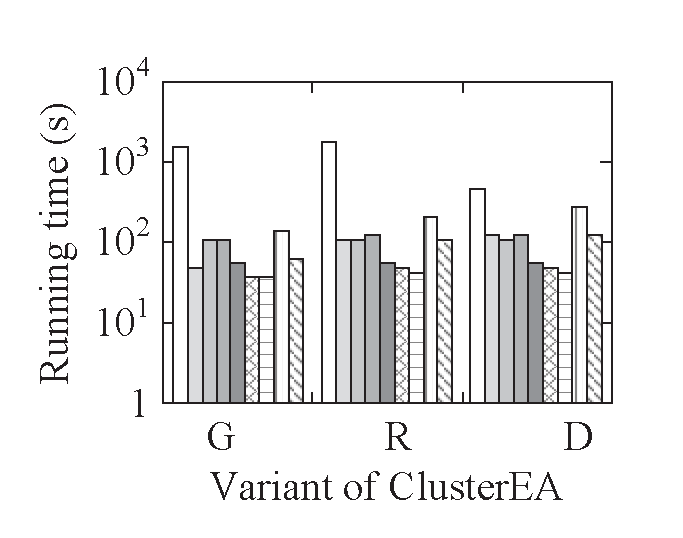
\includegraphics[width=1.55in]{figs/scalability-en-fr_1.eps}
}
% \hspace{-6mm}
\subfigure[EN-DE]{
 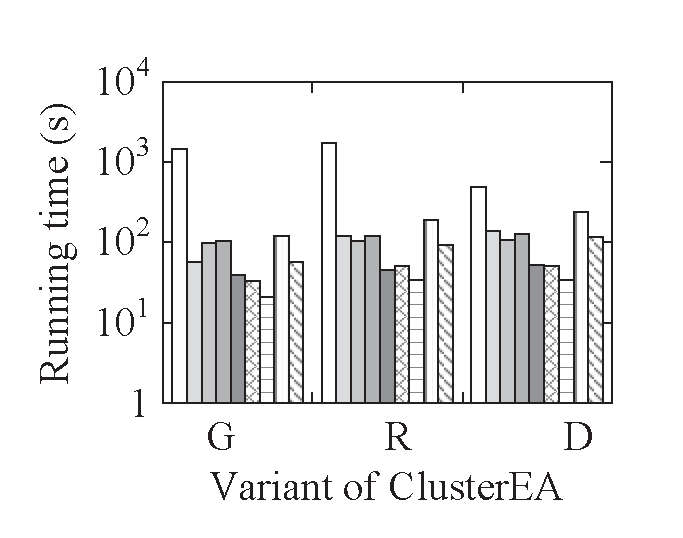
\includegraphics[width=1.55in]{figs/scalability-en-de_1.eps}
}
% \vspace*{-5mm}
\caption{Scalability analysis vs. variants of \ClusterEA{}}
% \vspace*{-3mm}
\label{fig:scalability}
\end{figure}
To further investigate the scalability of our proposed \ClusterEA{} framework, we verify the running time of each components in different variants of \ClusterEA{} on the DBP1M dataset, including (1) \emph{Training time} of the EA model; (2) \emph{\KMeans{}} batch sampling time; (3) \emph{\MetisGCN{}} batch sampling time on both directions; (4) \emph{Local Similarity Normalization time} of the batches generated by each samplers, denoted as Norm(Sampler); (5) \emph{Calculating Global Similarity} time in \Merging{}; and (6) \emph{Fusing Global and Local Similarity} time in \Merging{}. 
% For the structure channel, we report the running time of the mini-batch generation strategy (i.e., METIS-CPS) and that of EA model training.
The experimental results are shown in Figure~\ref{fig:scalability}, where G, R, and D denote \ClusterEA{-G}, \ClusterEA{-R}, and \ClusterEA{-D}, respectively. As depicted in Figure~\ref{fig:scalability}, we observe that the running time of each component except for Training time does not exceed $10^3$ seconds on the large-scale dataset.
This confirms the scalability of \ClusterEA{}. Note that the training time of the Dual-AMN model is significantly less than that of other variants. This is contributed by the model design of Dual-AMN that could dramatically reduce the required training epochs.
